\chapter{Kotlin Multiplatform}\label{ch:kotlin-multiplatform}

The Kotlin Multiplatform (KMP) technology allows developers to share code across multiple platforms, such as Android and iOS for mobile applications, and/or JVM, JavaScript and Native for multiplatform overall.


\section{Project Structure}\label{sec:project-structure}

A Kotlin Multiplatform project is divided into three main categories of code:

\begin{itemize}
    \item \textbf{Common}: Code shared between all platforms (i.e., \textit{CommonMain, CommonTest});
    \item \textbf{Intermediate}: Code that can be shared on a subset of platforms (i.e., \textit{AppleMain, AppleTest});
    \item \textbf{Specific}: Code specific to a target platform (i.e., \textit{\textless Platform\textgreater Main, \textless Platform\textgreater Test}).
\end{itemize}


An example of a Kotlin Multiplatform project architecture can be seen in Figure~\ref{fig:kmp-architecture}, but note that both \textit{Intermediate} and \textit{Specific} categories are optional.

\begin{figure}[H]
    \centering
    \caption{Example of a \textit{KMP} project architecture.}
    \label{fig:kmp-architecture}
    \vspace{0.3cm}
    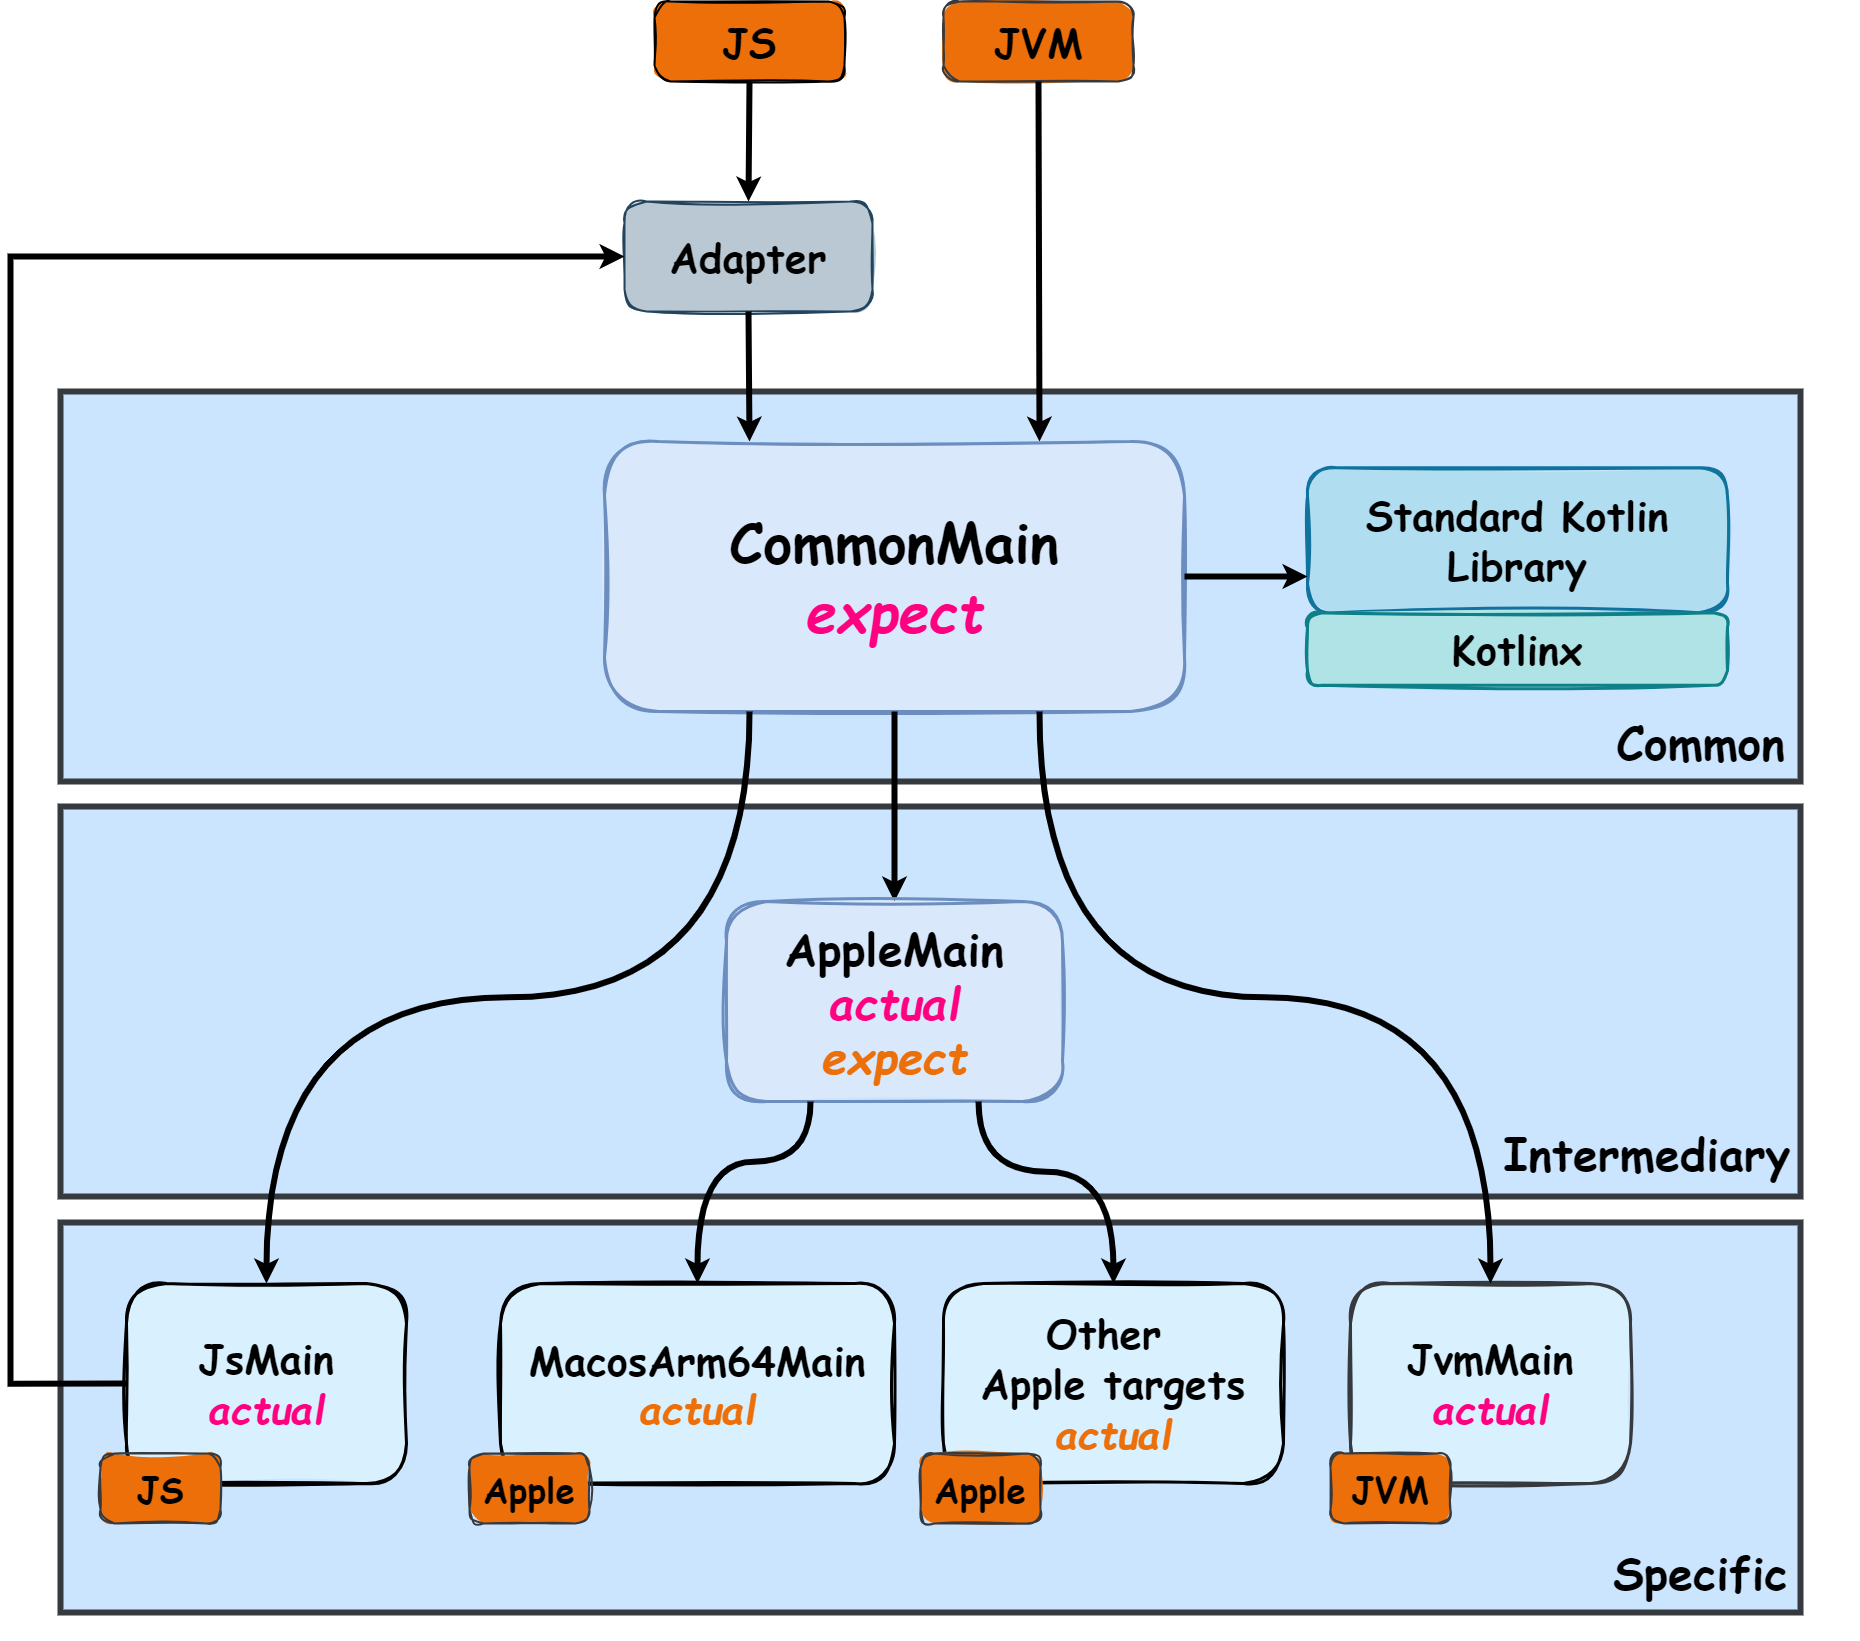
\includegraphics[width=1\textwidth]{../figures/02_kmp-architecture}
\end{figure}


Mention kotlin multiplatform project template github repository
Mention gradle project (divide in modules, gradle build file)


\section{Platform-Dependent Code}\label{sec:platform-dependent-code}

Since the main goal of \textit{KMP} is to share code across multiple platforms, the code should be written in a way that is as mutch platform-independent as possible (i.e., aggregating as much code as possible in the hierarchically superior categories).
However, it is sometimes necessary to create specific code for a given platform, regularly referred to as \textit{target}, in the following situations:

\begin{itemize}
    \item Access to API's specific to the \textit{target} is required (e.g., \textit{Java's File API});
    \item The libraries available in the common category (i.e., \textit{Standard Kotlin Library}, libraries from \textit{Kotlinx}) do not cover the desired functionalities and reducing third-party dependencies is a priority;
    \item A given \textit{target} does not directly support \textit{KMP} (e.g., \textit{Node.js)}, and so it is necessary to create an \textit{adapter}.
    This adapter allows communication with the common category code, in \textit{Kotlin}, from the native code of the \textit{target}, which can be defined in the \textit{Intermediate} or \textit{Specific} category.
\end{itemize}

To create specific code for a \textit{target} or subset of platforms, the mechanism \textbf{\textit{expect/actual}}~\cite{kmp-expect-actual} is used.
This mechanism allows defining the code to be implemented in an abstracted way and its implementation, respectively.


\section{Running Tests}\label{sec:running-tests}


\section{Other Aspects}\label{sec:other-aspects}
What was done to have concurrency, logging, CI integration, etc

